\documentclass[prl,12pt,onecolumn,nofootinbib,notitlepage,english,superscriptaddress]{revtex4-1}
\renewcommand{\rmdefault}{cmr}
\usepackage[T1]{fontenc}
\usepackage[latin9]{inputenc}
\setcounter{secnumdepth}{2}
\setcounter{tocdepth}{2}
\usepackage{color}
\usepackage{babel}
\usepackage{latexsym}
\usepackage{float}
\usepackage{amsmath}
\usepackage{amsfonts}
\usepackage{graphicx}
\usepackage{times}   %% Times Roman font
\usepackage{esint}
\usepackage{subfigure}
\usepackage{verbatim}
\usepackage{braket}
\usepackage{footmisc}
\usepackage[unicode=true,pdfusetitle,
 bookmarks=false,colorlinks=true,citecolor=blue,urlcolor=blue,linkcolor=red]{hyperref}
\makeatletter
%%%%%%%%%%%%%%%%%%%%%%%%%%%%%% LyX specific LaTeX commands.
\special{papersize=\the\paperwidth,\the\paperheight}

%%%%%%%%%%%%%%%%%%%%%%%%%%%%%% Textclass specific LaTeX commands.
\@ifundefined{textcolor}{}
{%
 \definecolor{BLACK}{gray}{0}
 \definecolor{WHITE}{gray}{1}
 \definecolor{RED}{rgb}{1,0,0}
 \definecolor{GREEN}{rgb}{0,1,0}
 \definecolor{BLUE}{rgb}{0,0,1}
 \definecolor{CYAN}{cmyk}{1,0,0,0}
 \definecolor{MAGENTA}{cmyk}{0,1,0,0}
 \definecolor{YELLOW}{cmyk}{0,0,1,0}
}

\@ifundefined{date}{}{\date{}}
\AtBeginDocument{
  \def\labelitemi{\(\rhd\)}
}
\makeatother

\setlength{\belowcaptionskip}{-7pt}
\newcommand{\SAVE}[1]{}
\newcommand{\HJC}[1]{{\color{RED}{\bf HJC: #1}}}
\newcommand{\prlsec}[1]{\emph{#1---}}
\newcommand{\Ncal}{{\mathcal N}}
\newcommand{\T}{{\mathbf{T}}}
\newcommand{\Jbq}{{J_{bq}}}
\newcommand{\DK}[1]{{\color{BLUE}{\bf DK: #1}}}

\begin{document}
\renewcommand{\thefootnote}{\fnsymbol{footnote}}
\renewcommand\abstractname{}
\title{From real materials to model lattice Hamiltonians: multi-scale modelling of strongly correlated electronic systems 
       with information from many body wavefunctions}

\author{Hitesh J. Changlani}
\affiliation{Department of Physics and Astronomy, Johns Hopkins University, Baltimore, Maryland 21218, USA}
\author{Huihuo Zheng}
\affiliation{
Argonne Leadership Computing Facility, Argonne National Laboratory, 9700 South Cass Avenue, Lemont, 60439, Illinois, USA}
\author{Brian Busemeyer}
\affiliation{Department of Physics and Institute for Condensed Matter Theory, University of Illinois at Urbana-Champaign, 
1110 West Green St, Urbana IL 61801, USA}
\author{Kiel Williams}
\affiliation{Department of Physics and Institute for Condensed Matter Theory, University of Illinois at Urbana-Champaign, 
1110 West Green St, Urbana IL 61801, USA}
\author{Lucas K. Wagner}
\affiliation{Department of Physics and Institute for Condensed Matter Theory, University of Illinois at Urbana-Champaign, 
1110 West Green St, Urbana IL 61801, USA}
\date{\today}
\maketitle

\textbf{
Given a realistic material with all its intrinsic complications, how does one develop a 
simple reliable model for understanding its properties? Theoretical insight has been the key driver of 
this process leading to simple few-band pictures. When the interactions are comparable 
to or much stronger than the kinetic energy, it is convenient to adopt the real space lattice 
approach and think in terms of Hubbard or Kanamori type Hamiltonians involving only the low energy electrons. 
But this is no easy task, since the effective Hamiltonian involves a considerable renormalization of parameters with respect 
to the bare Coulomb values. While the kinetic energy is dominated by contributions from bands or states energetically 
near the Fermi level, screened interactions depend on states even \emph{far} away from it, leading to Hubbard U's 
that have been traditionally hard to reliably determine. 
Here we discuss an approach that treats the kinetic and potential parts of the Hamiltonian 
democratically and one that provides a transparent way of obtaining effective Hamiltonians using data from many body wavefunctions, 
and whose validity can be systematically checked.
We emphasize that determining the effective Hamiltonian reliably is crucial for 
several applications in physics and chemistry not only for quantitative accuracy, but also a 
correct qualitative picture of strongly correlated materials. 
}

\section{Introduction to downfolding the many electron problem}

%\HJC{Survey of DFT based downfolding and known limitations....Survey of model Hamiltonians - Hubbard, Kanamori, .....}
%\HJC{Modify intro - this is from the paper........ }
%\HJC{How are many body systems studied, coarse graining - physics/ chemistry perspectives}
One of the most sought-after, yet often daunting endeavors, for physicists is to develop 
an intuitive understanding of physical phenomena involving intrinsically complicated materials 
using simplified models. These models are expected to capture the essence of the physics, and are formulated in terms 
of the most relevant physical degrees of freedom related to the observed phenomena. 
For example, at high temperature and low density when quantum effects are relatively insignificant, the ideal gas model 
successfully captures the statistical properties of $10^{23}$ H$_{2}$ molecules in a box, 
without any detailed knowledge of the fundamental constituent of H$_{2}$. This approach is valid when we are interested in 
phenomena at certain energy scale (or length scale), while the degrees of freedom at other length scales which are not 
dynamically excited simply renormalize the dynamics of the low energy degrees of freedom. 

This principle has also been widely employed in condensed matter physics. In the past few decades, several studies 
have been dedicated to describing complex systems (for example, the high $T_c$ cuprates and other transition metal oxides), 
in particular to strongly correlated systems. These are systems where the effects of Coulomb 
interactions are comparable to or more important than the kinetic energy and the picture of 
localized rather than itinerant electrons is more pertinent. This has motivated an approach beyond the 
traditional band theory approach, involving model Hamiltonians such as the Hubbard~\cite{Hubbard}, t-J~\cite{tJSpalek} 
and Heisenberg models, defined only in terms of the valence electrons. 
While these models have been extensively studied analytically and numerically, and have significantly 
enhanced our understanding of strongly correlated physics, their effectiveness 
for describing a real complex system of interest is often unclear. Since multiple 
competing energy scales are involved, rich phase diagrams emerge under a variety of conditions - doping, pressure, 
temperature, all heavily dependent on material-specific properties. This motivates 
the need to determine reliable low energy effective Hamiltonians that can capture all the necessary details, while 
remaining simple enough to be simulated accurately.  

%In complex systems such as high $T_c$ cuprates, it is unclear to what extent can these models describe the reality \cite{Anderson2013}. 
%Since strongly correlated systems are  the macroscopic phenomena are strongly dependent on material-specific properties, motivating the need to determine the effective Hamiltonians that can capture all necessary details. 
%In strongly correlated systems, the macroscopic phenomena are strongly dependent on material-specific properties, motivating the need to determine the effective Hamiltonians that can capture all necessary details. 
%\HJC{Downfolding: How should we connect our intuitive understanding of coarse graining with condensed matter concepts}
%The reliable simulation of strongly correlated systems remains a major challenge in physics, chemistry, and materials science. 
%On the other hand are approximate model Hamiltonians (such as the Hubbard model) 
%which describe the low energy physics solely in terms of the valence electrons and 
%are crucial to our understanding of physical phenomena such 
%as antiferromagnetism and high temperature superconductivity. 
%However, transitioning from actual materials to an effective Hamiltonian on a lattice relies 
%on physical insight and/or fits to experimental data, and this notion is not always rigorously well justified.

The endeavor we pursue here is a multi-scale approach in which the effective interactions between 
quasiparticles (such as dressed electrons) are determined after a full \emph{ab-initio}  
solution of the continuum Schroedinger equation involving all the electrons. This reduction 
of the Hilbert space is known as ``downfolding". This "lattice model" can be efficiently and accurately 
solved using techniques suited to small local Hilbert spaces- these include 
the density matrix renormalization group (DMRG), tensor networks~\cite{Verstraete,Changlani_CPS,Neuscamman_CPS}, 
dynamical field theory (DMFT), density matrix embedding (DMET) and lattice quantum Monte Carlo (QMC) methods. 
These methods have also been used to obtain excited states and dynamical correlation functions, that 
have been difficult in \emph{ab-initio} approaches. 
Full \emph{ab-initio} calculations are not computationally feasible for large system sizes 
and often not accurate enough to yield an unbiased understanding of the low energy states. 

Downfolding has most commonly been carried out using DFT-based approaches, 
most prominently the constrained-RPA approach. The hopping (kinetic) part is obtained from a standard 
DFT calculation which gives an estimate of the effective kinetic Hamiltonian. 
To estimate the interactions, one assumes a simple model of screening (based on RPA, for example) involving 
the Kohn Sham orbitals. Since some of the effects of the orbitals (one body space) have already been 
accounted for, the so called "double counting correction" is applied to obtain the downfolded Hamiltonian. 
Unfortunately, the formalism does not support a systematic way of internally 
checking the accuracy of the approximation, without resorting to comparison with experiment.  

Other downfolding approaches include traditional Lowdin downfolding 
within a stochastic approach and canonical transformation theory, 
also being actively pursued as a full fledged quantum chemistry method. 

Here we develop and apply a new set of methods which by nature of their formulation restore the democracy 
between kinetic and potential part of the Hamiltonian. 
While our method applies to any wavefunction based method, 
we have chosen the \emph{ab-initio} QMC approach~\cite{Ceperley_Alder,Foulkes_review}, 
due to its accuracy. The QMC method works directly in the continuum and 
explicitly introduces correlation into the Slater determinant obtained 
from DFT or Hartree Fock calculations. For energies of eigenstates, obtained 
by stochastic projection, the only systematic error is in the assumption of the 
nodes of the many-body wavefunction: in practice, 
this approximation is estimated to miss $ 5 - 10 \%$ 
of the correlation energy. Correlation functions and density matrices are generally 
less accurate, but good wavefunctions can bring down the errors significantly. 
For arbitrary wavefunctions which can be evaluated in polynomial time, 
the \emph{only} error is purely statistical and 
can be brought down to arbitrarily small values by increased sampling.

Information from many-body wavefunctions detects 
inadequacies of a proposed model: the deviations suggest the form of additional missing terms. 
Crucially, a wavefunction-based method does not differentiate between kinetic 
and potential energy terms: all terms are treated the same way. 
The approach is complementary to semi-empirical methods that 
fit models solely to available energy spectra. 

\section{Theory: Compression of the Energy Functional/Criteria for Hamiltonian matching}
\HJC{Lucas handling this section......Look at theory.tex}

%\HJC{What principles are important for connecting a problem of many electrons to a problem of few electrons}
%\HJC{Focus on density matrices and emphasize the reduction in number of effective orbitals. A dual problem: get the optimal one body space and also get the optimal effective interactions.}
%\HJC{Include Lucas' perspective}
%Our aim is to obtain a low energy effective Hamiltonian defined in 
%the active space of electrons which is preferably (but not necessarily) 
%described in terms of localized orbitals. In this basis, the criteria any 
%effective low energy model Hamiltonian must satisfy are,
%\begin{itemize}
%\item (a) The reduced density matrices (RDM) of the ground and excited states (computed in a basis) 
%          obtained from the \emph{ab-initio} calculation must match with that of the model calculation. 
%
%\item (b) The energy spectra of the \emph{ab-initio} and model systems must match in the energy window of interest. 
%
%\item(c) The model must be simple enough and must contain the essential physics to avoid over-parameterization and over-fitting. 
%\end{itemize}
%
%\HJC{Explain criterion 1}
%The concept of matching RDMs, criterion (a), 
%has previously appeared in related contexts~\cite{Acioli,Zhou_Ceperley, Changlani_percolation} 
%and in work by one of us~\cite{Wagner_JCP}. Most physical properties, 
%such as the charge and spin structure factors, are functions of the 2-RDM.
%Practically, it may be computationally expensive to get 
%high-order RDMs: in this study we use the matching condition only on the 
%2-RDM $\rho_{ijkl} \equiv \langle c_i^{\dagger} c_j^{\dagger} c_l c_k \rangle$ where $i,j,k,l$ are orbital indices 
%(including space and spin)
%\HJC{Note that good quantum numbers such as 
%total spin and angular momentum of a pure state are functions of the \emph{full} 
%2-RDM (if the Hamiltonian has those same symmetries) and not the \emph{partial} ones we use for matching.}.
%This criterion automatically ensures that 
%the combined number of electrons occupying the orbitals 
%is equal to those in the model Hamiltonian. (If any 
%input state does not satisfy the condition of 
%expected electron number, then it can not be described by the effective Hamiltonian.)  
%
%\HJC{Explain criterion 2}
%The importance of excited state energies 
%used in the fitting, criterion (b), is easily highlighted by the fact that 
%the wavefunctions (and hence their two-body density matrices) 
%are invariant to many kinds of terms that enter the Hamiltonian.
%For example, the transformation, 
%\begin{equation}
%	H' \rightarrow H + \alpha S^2 + \beta n + \gamma S^2 n 
%\end{equation}
%is, by construction, consistent with all the 2-RDM data 
%for any $\alpha$, $\beta$, $\gamma$ 
%for systems which have spin symmetry and conserve particle number.
%Imposing certain "physical constraints" on the form of the 
%interactions can eliminate the need for this criterion. 
%To give a concrete example, consider wavefunction data 
%generated from the ground state of an unfrustrated 
%Heisenberg Hamiltonian in a bipartite lattice~\HJC{A bipartite 
%lattice is one with two sublattices $A$ and $B$ with 
%only $A-B$ connections but no $A-A$ or $B-B$ ones.}, 
%$ H = J \sum_{\langle i,j \rangle}\bar{S}_i \cdot \bar{S_j}.$ 
%where $\langle i,j \rangle$ refer to nearest neighbor pairs.
%Then adding $\alpha S^2$ gives the same correlators (density matrices) 
%of the ground state, as long as $\alpha$ is small enough to not cause 
%energy crossings i.e. not make an original 
%excited state the new ground state. This additional 
%term has the effect of introducing long range Heisenberg couplings. 
%Moreover, the effective Hamiltonian is not unique: 
%the Lieb-Mattis model~\cite{LM} $H = S_A \dot S_B$ 
%(where $A$ and $B$ refer to sublattice spins), is also 
%known to reproduce the low-energy limit of the Heisenberg model. 
%Thus, imposing the requirement that the Hamiltonian has the 
%nearest-neighbor form constrains $\alpha$ to zero and picks 
%one particular model. Similar arguments should 
%apply to long-range Hubbard models in homogeneous 
%systems where a physical constraint is that density-density 
%interaction must decrease monotonically with distance between orbitals. 
%
%While having many excited states from \emph{ab-initio} calculations 
%is desirable, we note that certain methods only work best for 
%determining ground states in symmetry sectors. 
%In the case of FN-DMC, 
%some other excited states can also be achieved by fixing their 
%nodal structure (which is different from that of the ground state). 
%Our practical experience suggests that attempts to obtain 
%eigenstates were often associated with broken symmetries. 
%This happens for a variety of reasons: choice of DFT orbitals, 
%contamination of the spin-structure by the 
%Jastrow and/or incomplete optimization. 
%These limitations suggest that it is 
%important to reduce the dependence of the desired 
%method only on eigenstates. Instead, our philosophy is to 
%use the \emph{available} information from arbitrary 
%low-energy states to our advantage. 
%(Moreover, if \emph{all} eigenstates were known, the utility of 
%generating an effective Hamiltonian might be diluted anyway.)
%  
%Given a finite amount of data, we note that criteria (a) and (b) 
%do not always uniquely determine an effective Hamiltonian, 
%even within the ansatz chosen. For example, one may demand that 
%the cross expectation values of certain operators 
%(say $\langle \psi_1 | c_i^{\dagger} c_j | \psi_2 \rangle$) 
%between the \emph{ab-initio} and model calculations must match. 
%This information could also be added as an 
%additional criterion for matching. 
%
%\HJC{Importance of transferability}
%Finally, it is important to build confidence 
%in this Hamiltonian by comparing its outputs with respect 
%to data not used in the fitting. 
%To partly remedy this, we propose the 
%heuristic criterion (c). As is the case with many situations 
%involving fitting, we desire 
%the minimal model that explains the data to 
%some reasonable accuracy. This has the effect of making such a 
%model Hamiltonian useful in other situations i.e. transferable.
%
%\HJC{Hubbard parameters are fit parameters, do not have any deep meaning necessarily.}
%What is the meaning of the Hubbard $U$ (and other interactions)?
%Is there a fundamental definition or are they fit parameters to a chosen model? 
%We take the latter viewpoint and thinking this way helps reconcile 
%widely varying estimates that exist in the literature. 
%A common expression for the generalized-two body interaction is taken to be, 
%\begin{equation}
% V_{ijkl} = \int  \phi_i (r) \phi_j (r')  W (r,r') \phi_k (r) \phi_l (r')
%\end{equation}
%where the modified interaction $W(r,r')$ is obtained from a model for screening 
%relating it to the bare Coulomb interaction $V(r,r')$. 
%
%
%\subsection{Choice of 1 particle orbitals, energy window, data selection...etc}
%\HJC{IAO, Wannier or something else?}
%
%\HJC{Choice of energy window - Hubbard parameters could be energy dependent. Static vs dynamic (energy dependent) 
%models.}
%The Hubbard $U$ depends on the energy range 
%over which one is interested in estimating it. It is an 
%"effective interaction" that encodes the effect of many others 
%which would otherwise be needed in a completely static model.
%Even in the low frequency static limit, estimates 
%of the Hubbard $U$ can vary over large factors~\cite{Fei_Lin} 
%(of the order of $2$ or more): this is partly attributed to insensitivity 
%of correlation-functions in the ground state to its precise value. 
%Any inaccuracy in the \emph{ab-initio} calculation reflects as 
%large changes in the estimated $U$. This point 
%will become clearer in later sections of the paper.
% 
%\HJC {What kind of data is needed and how much is enough}
%In the fitting approach, the idea is to use a sufficiently 
%large data set such that the proposed Hamiltonian has "learnt" most 
%relevant features of the low-energy physics, after which the parameters 
%are used for understanding other properties. 
%This reconstruction depends on the kind of data input to the method 
%and the presence of linear dependencies. 
%We present a formulation which puts the statements above 
%on a more rigorous mathematical footing.
%
%\HJC {Given data, how do we achieve what we want...}
%\subsection{Fitting procedure: $Ax=E$ method}
%\label{sec:AxE}
%Consider a set of \emph{ab-initio} 
%energies $E_s$ (in general, expectation values of the Hamiltonian) 
%and corresponding 1 and 2 body RDMs $\langle c_i^{\dagger} c_j \rangle_s$ 
%$\langle c_i^{\dagger}c_j^{\dagger} c_l c_k \rangle_s$ 
%for various \emph{arbitrary} low-energy states characterized by index $s$. 
%Assume a model 2-body Hamiltonian parameterized by (yet unknown) 
%renormalized parameters $t_{ij}$ (one body part) 
%and $V_{i,j,k,l}$ (2-body part) along with a constant term $C$, 
%the total number of parameters being $N_p$. Then for each state $s$, 
%we have the equation, 
%\begin{equation}
%	E_s = \langle H \rangle_s = C + \sum_{ij} t_{ij} \langle c_i^{\dagger} c_j \rangle + \sum_{ijkl} V_{ijkl} \langle c_i^{\dagger}c_j^{\dagger} c_l c_k \rangle  
%\end{equation}
%where we have made the assumption that the chosen set of orbitals 
%is capable of explaining all energy differences. The constant $C$ is from energetic contributions 
%of all other orbitals which are (almost) decoupled from the chosen set.  
% 
%We then perform calculations for 
%$M$ (possibly random) low-energy states which are not necessarily eigenstates.  
%The objective is to explore various parts 
%of the low-energy Hilbert space which show variations in the 2-RDM elements. 
%Since the same parameters describe all $M$ states, they must 
%satisfy the linear set of equations, 
%\begin{eqnarray}
%\left(
%\begin{array}{c}
%E_1 \\
%E_2 \\
%E_3 \\
%... \\
%... \\
%... \\
%... \\
%E_M
%\end{array}
%\right) =
%\left(
%\begin{array}{ccccc}
%1 & \langle c_i^{\dagger}c_j \rangle_{1}  & .. & \langle c_i^{\dagger}c_j^{\dagger}c_l c_k \rangle_{1} & .. \\
%1 & \langle c_i^{\dagger}c_j \rangle_{2}  & .. & \langle c_i^{\dagger}c_j^{\dagger}c_l c_k \rangle_{2} & .. \\
%1 & \langle c_i^{\dagger}c_j \rangle_{3}  & .. & \langle c_i^{\dagger}c_j^{\dagger}c_l c_k \rangle_{3} & .. \\
%1 & \langle c_i^{\dagger}c_j \rangle_{4}  & .. & \langle c_i^{\dagger}c_j^{\dagger}c_l c_k \rangle_{4} & .. \\
%1 & ....                                  & .. & ..                                                    & .. \\
%1 & ....                                  & .. & ..                                                    & .. \\
%1 & \langle c_i^{\dagger}c_j \rangle_{M}  & .. & \langle c_i^{\dagger}c_j^{\dagger}c_l c_k \rangle_{M} & .. \\
%\end{array}
%\right) \left(
%\begin{array}{c}
%C           \\
%t_{ij}      \\
%..          \\
%V_{ijkl}    \\
%..
%\end{array}
%\right)
%\end{eqnarray}
%which can be written more compactly as,
%\begin{equation}
%	{\bf{E}} = A {\bf{x}}
%\end{equation}
%where $ {\bf{E}} \equiv (E_1,E_2,...E_M)^{T}$ 
%is the $M$ dimensional vector of energies, $A$ is the $M \times N_p$ matrix composed 
%of density matrix elements and $ {\bf{x}} \equiv (C,t_{ij}....V_{ijkl}...)^T$ 
%is a $N_p$ dimensional vector of parameters.
%This problem is overdetermined for $M>N_p$, which is the regime we expect to work in.
%
%In the case of any imperfection in the model (which is the most common case), 
%the equality will not hold exactly 
%and one must then instead minimize the norm, $\mathcal{N}$,
%\begin{equation}
%	\mathcal{N} \equiv ||A\bf{x}-\bf{E}||^2
%\label{eq:norm}
%\end{equation}
%The nice property of this cost function is that it can be minimized
%in a single step by using the method of least squares, employing the singular 
%value decomposition of matrix $A$, which also encodes exact (or near-exact) linear dependences. 
%Thus, the quality of the fit can be directly judged 
%by assessing (1) the singular values of the $A$ matrix and (2) 
%the value of the cost function itself i.e. the deviations of the input and fitted energies.
%We will refer to this method as the "Ax=E" method at various points in the paper.
%
%\HJC{Advantage over other cost functions... L1 norm may not be so nice but it could give more minimal models?}
%The cost function~\eqref{eq:norm} is unlike that used when matching 
%canonical density operators,
%\begin{equation} 
%\frac{1} {Z^{m}} \exp(-\beta H^{m})  = \frac{1} {Z^{a}} \exp(-\beta H^{a})
%\label{eq:Z_Zstar}
%\end {equation}
%where indices $m$ and $a$ refer to the model and ab-initio (true) systems, $\beta$ 
%is an inverse temperature and $Z$ is the partition function
%In contrast, our "energy-weighting" function is a box-function: it weighs all the energies 
%in a given window equally. The form of the cost function (including the 
%weighting function) is unimportant in the limit of a perfect model.
%
%In summary, our approach solves 
%linear equations in terms of the unknown parameters, by using the density matrices 
%from an \emph{ab-initio} method. This concept works only when we 
%know the model Hamiltonian that describes the data, and all we want is the numerical 
%values of the parameters. Thus to verify the validity of the calculation, 
%one must use the derived parameters and calculate many-body eigenstates 
%in the model and check their correspondence with the \emph{ab-initio} 
%calculations.
%
%\HJC{What does the A matrix encode - standard tricks of fitting...}
%The matrix $A$ gives a very natural basis to understand "renormalization" effects.
%For example, consider a set of wavefunctions, that show that the correlator 
%$\langle n_0 n_3 \rangle$ does not change significantly. This would lead to the 
%corresponding column of matrix $A$ being identical (up to a scale factor) 
%to the first column of 1's. Physically, this would correspond to the coupling constant 
%$V_{03}$ being unimportant (it can take any value including 0) and its 
%effect can be completely absorbed into the constant shift term. 
%(This could also alternatively mean that the input 
%data is correlated and does not provide enough information about $V_{03}$. 
%In the case of non-zero "small variations", the value of this parameter 
%will be quite sensitive to the data set and its quality.) 
%Said differently, it is the \emph{variation}  
%in an RDM element (across states in the energy window) 
%that are important: \emph{not} their \emph{absolute} values.
%
%\subsection{QMC specific features}
%\HJC{Till this point perfectly general... QMC helps.... etc etc}
%The utility of the wavefunction approach is apparent in this 
%formulation: the expectation values entering matrix $A$ 
%can be calculated for arbitrary wavefunctions by Monte Carlo sampling.
%We can also simply use variational Monte Carlo and corresponding energies
%for constructing the $A$ matrix, however we may not get the desired accuracy. 
%
%\HJC{QMC specific}
%It is thus preferable to use the accurate FN-DMC method. In this case, one needs to modify the linear equations 
%to use projected estimators. More specifically, we have, $E= \langle {\psi_T}^{s}| H | {\psi}^s \rangle$ 
%and thus must use the projected estimates of the density matrix elements i.e. 
%$\langle {\psi_T}^s | c_i^{\dagger} c_j | {\psi}^s \rangle$ and $\langle {\psi_T}^s| c_i^{\dagger}c_j^{\dagger} c_l c_k | {\psi}^s \rangle$ 
%in the construction of the $A$ matrix. (The implicit normalization of these 
%mixed estimates by $\langle {\psi_T}^s | \psi^{s} \rangle$ is assumed.) 
%This projector formulation is also very amenable to 
%coupled-cluster calculations which also work with projected energies 
%and density matrices.
%
%\HJC{QMC specific}
%There is no need to worry about the bias in FN-DMC in our formulation. 
%This is because we regard $\psi \psi_T$ as some \emph{arbitrary} positive sampling function 
%associated with a low energy state and use the \emph{same} distribution for the 
%evaluation of the density matrix elements. We are not concerned with whether 
%an exact eigenstate is being sampled or not: we just desire a linear equation 
%(for the unknown parameters) from this exercise. Thus the relationship between the FN-DMC energy 
%and the projected density matrix elements is always an \emph{exact} relationship 
%(up to errors coming in from statistics and from the 
%assumption of the form of the Hamiltonian). 


%\HJC{Visualizing the goodness of fit/connecting to tools from data science}
%\HJC{Choice of norm and avoiding over-fitting: $L_1$, $L_2$ or something else?}

\section{Representative Examples}
%\HJC{Choosing the optimal one body space/ Dual optimization of Hamiltonian parameters and basis sets}
%\HJC{Simple examples - lattice to lattice downfolding - Three to One band model and the "effective" d orbitals}
%\HJC{Notes on 3 band - copy pasted from pdf, tex file missing ?????}
\subsection{Three-band Hubbard model to one band Hubbard model at half filling}
%\HJC{What is the 3 band model? Why the 3 band model??}
\subsubsection{Introduction}
A big motivation for studying lattice models of strongly correlated systems comes from their 
relevance to the high $T_c$ superconducting cuprates~\cite{Bednorz1986}. These materials are complex, with several 
competing energy scales, leading to rich phase diagrams~\cite{Dagotto_RevModPhys, LeeWen_RevModPhys}. In these materials, 
the low energy physics is primarily associated with the copper-oxygen 2D planes. 
%(Inter-layer effects can also important for some aspects, a complication we ignore 
%for this work.) 

Many works have been devoted to determining the model effective Hamiltonians and corresponding parameter 
values for the cuprates~\cite{Emery, ZhangRice, tJSpalek, Hybertsen_PRB1989, Hybertsen_PRB1990, Pavirini, Kent_Hubbard}. 
Accounting for the octahedral environment of copper ions, and with support from electronic structure 
and quantum chemistry calculations~\cite{Dagotto_RevModPhys}, one infers 
that the five-fold \emph{d} orbital degeneracy of the isolated copper ion is lifted to make the 
highest filled orbital with one unpaired electron to be the one with $d_{x^2-y^2}$ character. 
(The choice of spatial coordinates corresponds to the copper oxide plane to be the X-Y plane). 
The corresponding oxygen orbitals that hybridize most strongly with this orbital are the $p_x$ or $p_y$ orbitals. 
Thus the minimal model for the cuprates involving the oxygens 
is the 3-orbital or 3-band Hubbard model, 
\begin{eqnarray}
H &=&    \epsilon_p \sum_{j,\sigma} \epsilon_p n^{p}_{j,\sigma} + \epsilon_{d} \sum_{d}  n^{d}_{i,\sigma} 
	+ t_{pd} \sum_{\langle i,j \rangle, \sigma} \text{sgn}(p_i,d_j) \Big( d_{i,\sigma}^{\dagger} p_{j,\sigma} + \text{h.c.} \Big) \\
  & &   + U_p \sum_{j} n^{p}_{j,\uparrow} n^{p}_{j,\downarrow} + U_d \sum_{i} n^{d}_{i,\uparrow} n^{d}_{i,\downarrow} + V_{pd} \sum_{\langle i,j \rangle} n^{j}_p n^{i}_d 
\end{eqnarray}
where $d_i,p_j$ refer to the orbitals of copper (at site $i$) and oxygen (at site $j$)  respectively 
and the signs of the hopping $t_{pd}$ between them is shown in Fig.~\ref{fig:threeband} for a $2 \times 2$ unit cell. 
$\epsilon_p$,$\epsilon_d$ refer to the orbital energies, 
$U_d$, $U_p$ refer to strength of onsite Hubbard interactions and $V_{pd}$ refers to the 
stength of the density-density interactions between a neighboring $p$ and $d$ orbital. 
One could consider further variations of the model by adding $t_{pp}$ type hoppings, but 
these have not been shown here. To keep the exposition simple, we consider only 
the case where $\epsilon_p$, $t_{pd}$ and $U_{d}$ are non zero and 
since we work with a fixed number of particles, set $\epsilon_d = 0$. Thus the 
charge transfer energy $\Delta \equiv \epsilon_p - \epsilon_d$ equals $\epsilon_p$ in our notation. 

\begin{figure}[htpb]
\centering
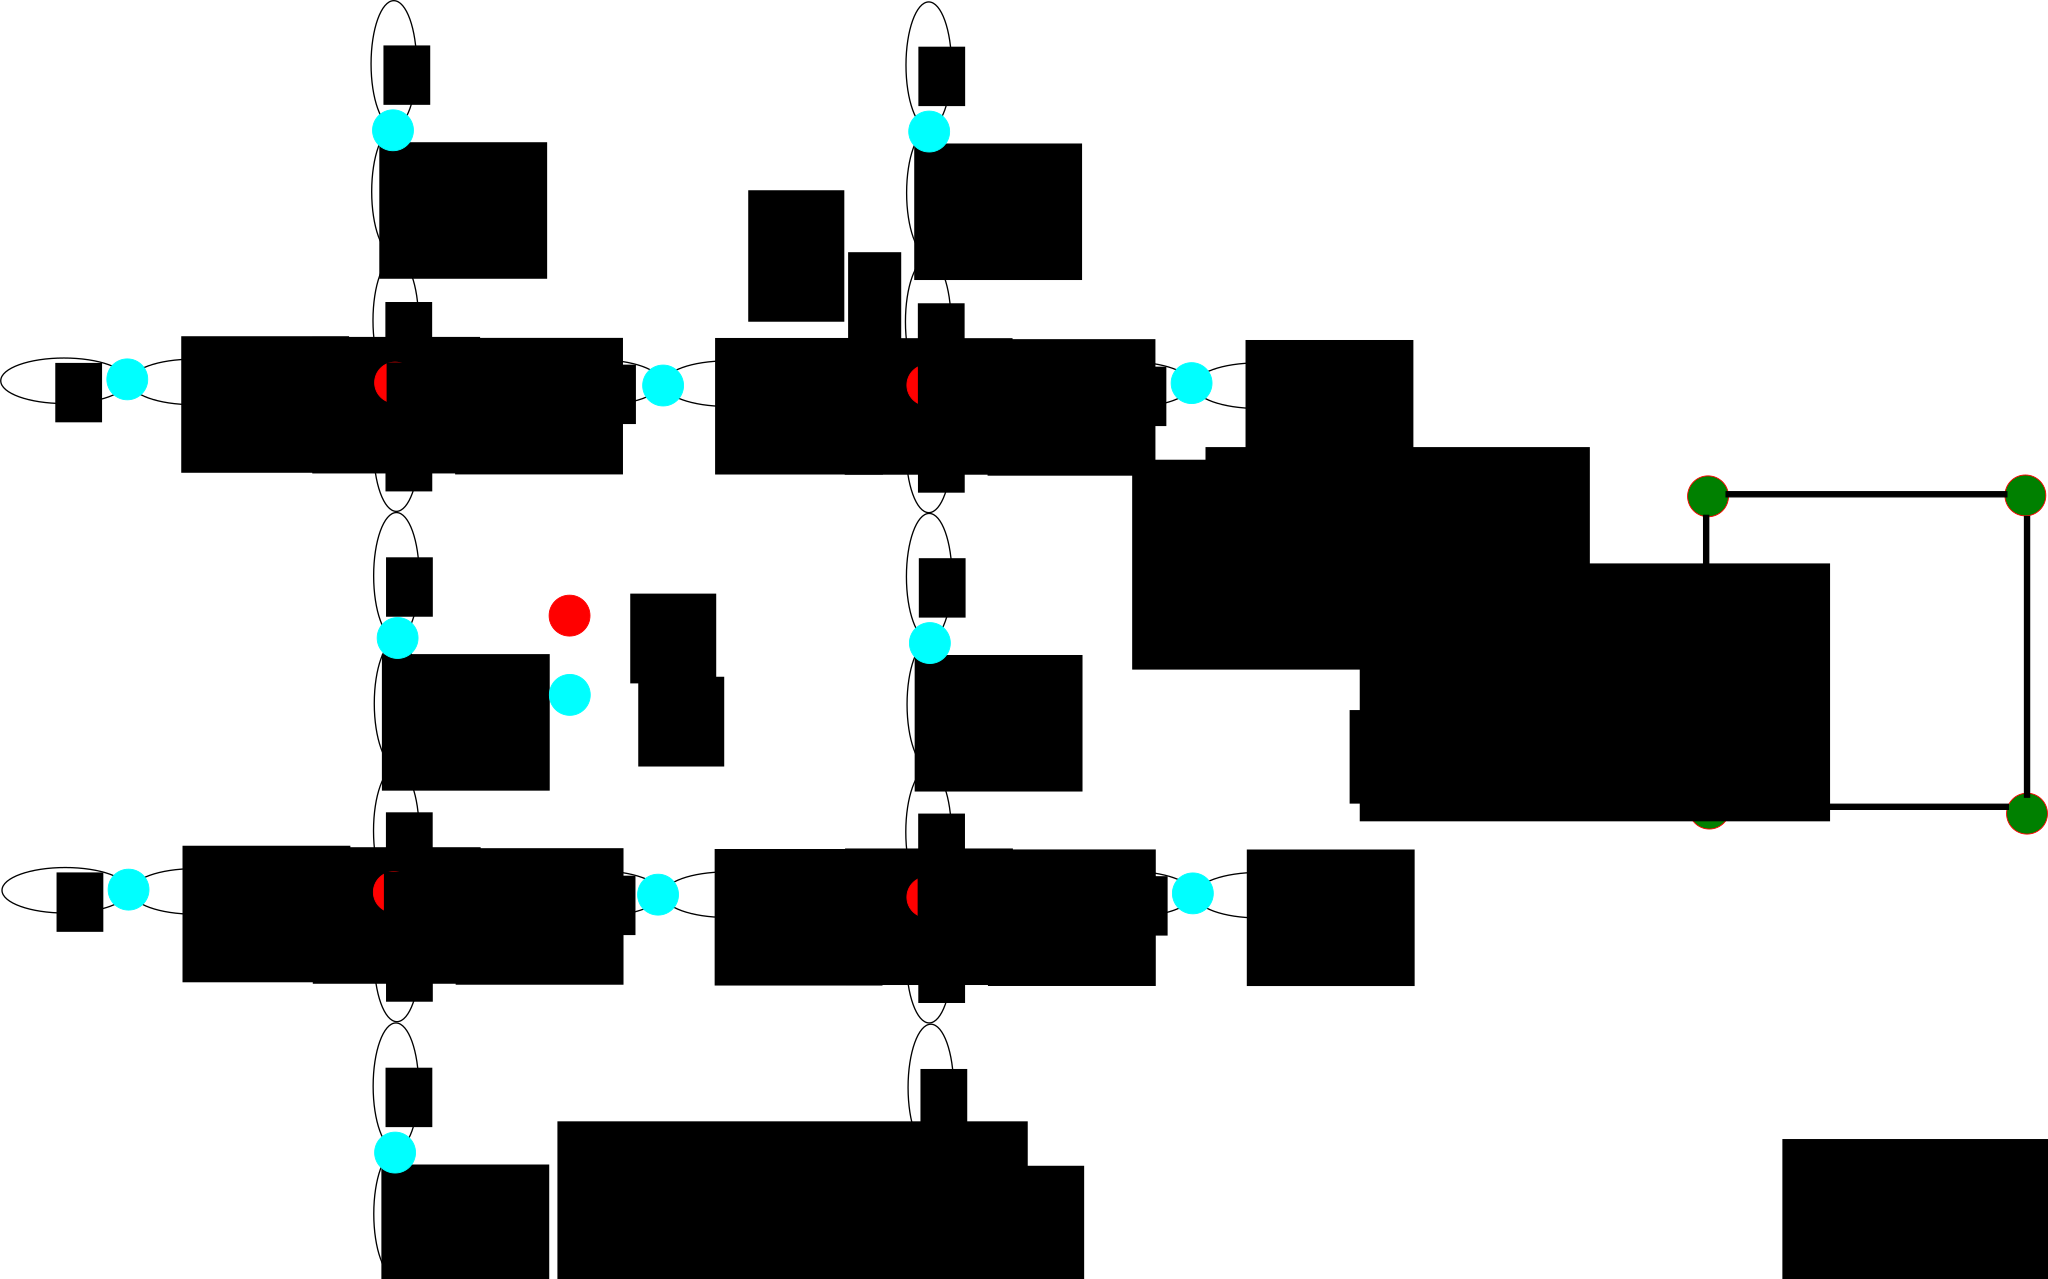
\includegraphics[width=1\linewidth]{./three_band_figure.pdf}
\caption{Schematic for downfolding the three band Hubbard model to the one band Hubbard model. 
The oxygen orbitals are completely eliminated to give "dressed" $d$-like orbitals of the one band model, with modified hopping 
and interaction parameters.}
\label{fig:threeband} 
\end{figure}	

The justification for the 3-band model for the cuprates, along with the determination of its parameters, 
is itself contingent on downfolding from a wavefunction based \emph{ab-initio} calculation, 
of the type carried out in Refs.~\cite{Wagner_Abbamonte}. There has also been a suggestion that the 4s orbital of copper is important 
for the low energy properties~\cite{Pavirini} but we steer clear of this debate here. 
Instead we use the 3-band model at half filling, as a prototypical example of what it \emph{means} to downfold to 
a simpler model - the one band Hubbard model, 
\begin{eqnarray}
	\tilde{H} &=&  -t \;\sum_{\langle i,j \rangle} \tilde{d}_i^{\dagger} \tilde{d}_j + U \;\sum_{i} \tilde{n}^{i}_{\uparrow} \tilde{n}^{i}_{\downarrow}
\label{eq:oneband}
\end{eqnarray}
where $t$ and $U$ are downfolded (renormalized) Hubbard parameters, which are to 
be determined for given 3-band parameters, and $\tilde{d}$ are the effective \emph{d-like} orbitals. 
The latter are a mixture of copper and oxygen orbitals and this optimal transformation also remains an unknown. Thus, 
the determination of effective Hamiltonians is a \emph{dual} problem - (1) what are the composite objects that give a 
compact description of the low energy physics? and given this choice what are the effective interactions between them?  
This example will serve as a setting for the downfolding of more complex \emph{ab-initio} systems to lattice 
models. 
%\lucas{I don't know how much to trust these parameters, to be honest with you.} 
%\begin{table*}
%\begin{ruledtabular}
% \begin{tabular}{cccc}
%  Parameter				&  LE = Lucas (electron)    & LH = Lucas (hole) & SH = Shiwei (hole) \\ 
%	$t_{pd}$			&  $-1.31$		    & $+1.31$        &     $+1.00$ 	       \\
%	$t_{pp}$			&  $-0.90$		    & $+0.90$        &     $+0.00$	       \\
%	$U_{pd}$			&  $+0.00$		    & $+0.00$        &     $+0.00$ 	       \\
%	$U_{d}$				&  $+8.00$		    & $+8.00$        &     $+6.00$ 	       \\
%	$U_{p}$				&  $+1.79$		    & $+1.79$        &     $+0.00$ 	       \\
%        $\epsilon_{p}$			&  $+0.00$		    & $+0.00$        &     $+3.00$          \\
%        $\epsilon_{d}$			&  $-3.50$		    & $-2.71$        &     $+0.00$          \\
%$\Delta=\epsilon_{p}-\epsilon_{d}$      &  $+3.50$		    & $+2.71$        &     $+3.00$          \\
%  \end{tabular}
% \end{ruledtabular}
% \caption{Parameter sets. The sign of $t_{pd}$ does not matter in either notation because this sign can be absorbed 
%into the redefinition of the d orbital itself, see discussion on particle hole transformations. 
%Nevertheless we stick to the sign conventions above, unless otherwise mentioned.}
% \label{table:params}
%\end{table*}
%
%\HJC{How do we think of the problem...? effective d orbitals.... explain associated Figure}
%\HJC{Lot of stuff needs to be taken out or re-explained....}

\subsubsection{Choice of effective one particle basis}
To map the 3-band model to the 1-band model and determine its validity, 
our first aim will be to obtain effective "dressed" \emph{d-like} 
orbitals that enter Eq.~\ref{eq:oneband}. We encode this relationship as 
the transformation ${\bf T}$, 
\begin{equation}
	\tilde{d}_i^{\dagger} = \sum_{j} T_{ij} c_j
\end{equation}
where $\tilde{d}_i$ is a transformed hole operator and $c_j$ is the bare hole
operator, the latter could refer to either $d$ or $p$ orbitals. Accounting for all symmetries of 
the $2\times2$ unit cell, {\bf T} is a $4 \times 12 $ matrix (the numbering of the orbitals 
corresponds to Fig.~\ref{fig:threeband}) is explicitly written out as, 
\begin{eqnarray}
{\bf T} = 
\left(
\begin{array}{cccccccccccc}
F        & \alpha_2 &        \alpha_2 &  \alpha_4 & \alpha_1 & \alpha_1 & -\alpha_1 & -\alpha_1 & \alpha_3 & -\alpha_3 & \alpha_3 & -\alpha_3 \\
\alpha_2 &  F       &        \alpha_4 &  \alpha_2 & \alpha_3 & -\alpha_1 & \alpha_1 & -\alpha_3 & -\alpha_3 & \alpha_3 & \alpha_1 & -\alpha_1 \\
\alpha_2 & \alpha_4 & F               &  \alpha_2 & -\alpha_1 & \alpha_3 & -\alpha_3 & \alpha_1 & \alpha_1 & -\alpha_1 & -\alpha_3 & \alpha_3 \\
\alpha_4 & \alpha_2 & \alpha_2        &   F       & -\alpha_3 & -\alpha_3 & \alpha_3 & \alpha_3 & -\alpha_1 & \alpha_1 & -\alpha_1 & \alpha_1 \\
\end{array}
\right)
\end{eqnarray}
where we have defined $F \equiv \sqrt{1-4{\alpha_1}^2 - 2{\alpha_2}^2 - 4 {\alpha_3}^2 -{\alpha_4}^2}$ and 
where the parameters $\alpha_1$,$\alpha_2$,$\alpha_3$ and $\alpha_4$ will be 
optimized to minimize a certain cost function, which will be explained shortly. 

Note that the transformation has been chosen to be a linear one. One can imagine a more complicated 
many-body transformation involving higher body functions. In practice, at least for the model under 
consideration, this does not seem to be necessary. 
%This does not mean that determining the optimal one body space is \emph{always} a trivial problem. 
%In fact, (as pointed out to us by D. Ceperley) there are several interesting problems in the study of helium 
%that involve ring exchanges involving as many as 12 particles~\cite{Ceperley_Jacucci}, 
%certainly our simple minded transformation does not capture the search for such multi-body 
%or composite objects. However, for the purpose of the rest of the paper, we will show the utility 
%of the linear transformations even for the \emph{ab-initio} to lattice downfolding cases; 
%Kohn Sham orbitals will be rotated to form localized functions. These one body transformations will give us the orbitals 
%that enter the definition of the effective Hamiltonian. 

\begin{figure}[]
\centering
\includegraphics[width=0.49\linewidth]{./Hyb_vs_U_Ud_8.pdf}
\includegraphics[width=0.49\linewidth]{./Hopping_vs_U_Ud_8.pdf}
\includegraphics[width=0.49\linewidth]{./downfolded_U_Ud_8.pdf}
\caption{Downfolded values of the effective 1-band Hubbard U/t and hopping $t_{opt}$ vs $U_d/t_{pd}$}
\label{fig:hamfit} 
\end{figure}	

\begin{figure}[]
\centering
\includegraphics[width=0.49\linewidth]{./downfolded_U_ep_3.pdf}
\includegraphics[width=0.49\linewidth]{./downfolded_U_ep_5.pdf}
\includegraphics[width=0.49\linewidth]{./Hopping_vs_U_ep_3.pdf}
\includegraphics[width=0.49\linewidth]{./Hopping_vs_U_ep_5.pdf}
\caption{Downfolded values of the effective 1-band Hubbard U/t and hopping $t_{opt}$ vs $U_d/t_{pd}$}
\label{fig:hamfit} 
\end{figure}	

\begin{figure}[]
\centering
\includegraphics[width=0.325\linewidth]{./Gap_1_band_3_band_ep_3_number_5.pdf}
\includegraphics[width=0.325\linewidth]{./Gap_1_band_3_band_ep_3_number_9.pdf}
\includegraphics[width=0.325\linewidth]{./Gap_1_band_3_band_ep_3_number_2.pdf}
\includegraphics[width=0.325\linewidth]{./Gap_1_band_3_band_ep_5_number_5.pdf}
\includegraphics[width=0.325\linewidth]{./Gap_1_band_3_band_ep_5_number_9.pdf}
\includegraphics[width=0.325\linewidth]{./Gap_1_band_3_band_ep_5_number_2.pdf}
\caption{Comparison for energy gaps between the 3-band and 1-band Hubbard models using the optimized values of $U/t$ and $t$, for different
$U_{d}/t_{pd}$ for $\Delta/t_{pd}=3$ and $\Delta/t_{pd}=5$}
\label{fig:hamfit} 
\end{figure}	

The one particle density matrix in the transformed basis is related 
to that in the original basis by,
\begin{equation}
	\langle {\tilde{d}_i}^{\dagger} \tilde{d}_{j} \rangle = \sum_{mn} U^{*}_{im} \langle {c_m}^{\dagger} c_n \rangle U_{jn}
\end{equation}
and using this relationship we demand two conditions be satisfied,
\begin{itemize} 
 \item The effective orbitals are orthogonal to each other 
 \item All diagonal entries of the 1-RDM of the effective orbitals for all eigenstates 
       $(\langle \langle {\tilde{d}_i}^{\dagger} \tilde{d}_{i} \rangle \rangle)$ 
       equal 1/2 since, as we are working at half filling.
\end{itemize} 
We consider a cost function 

\subsubsection{Results and Discussion}
To give a concrete example of our results, we start with 1-RDM of the lowest eigenstate, 
\begin{eqnarray}
\left(
\begin{array}{cccccccccccc}
+0.380	   & -0.091 &-0.091 &-0.015& +0.119& +0.119& -0.119 &-0.119 &-0.017 &+0.017 &-0.017 &+0.017 \\
-0.091	   & +0.380 &-0.015 &-0.091& -0.017& -0.119& +0.119 &+0.017 &+0.017 &-0.017 &+0.119 &-0.119 \\
-0.091	   & -0.015 &+0.380 &-0.091& -0.119& -0.017& +0.017 &+0.119 &+0.119 &-0.119 &+0.017 &-0.017 \\
-0.015	   & -0.091 &-0.091 &+0.380& +0.017& +0.017& -0.017 &-0.017 &-0.119 &+0.119 &-0.119 &+0.119 \\
+0.119	   & -0.017 &-0.119 &+0.017& +0.060& +0.034& -0.034 &-0.060 &-0.034 &+0.034 &-0.007 &+0.007 \\
+0.119	   & -0.119 &-0.017 &+0.017& +0.034& +0.060& -0.060 &-0.034 &-0.007 &+0.007 &-0.034 &+0.034 \\
-0.119	   & +0.119 &+0.017 &-0.017& -0.034& -0.060& +0.060 &+0.034 &+0.007 &-0.007 &+0.034 &-0.034 \\
-0.119	   & +0.017 &+0.119 &-0.017& -0.060& -0.034& +0.034 &+0.060 &+0.034 &-0.034 &+0.007 &-0.007 \\
-0.017	   & +0.017 &+0.119 &-0.119& -0.034& -0.007& +0.007 &+0.034 &+0.060 &-0.060 &+0.034 &-0.034 \\
+0.017	   & -0.017 &-0.119 &+0.119& +0.034& +0.007& -0.007 &-0.034 &-0.060 &+0.060 &-0.034 &+0.034 \\
-0.017	   & +0.119 &+0.017 &-0.119& -0.007& -0.034& +0.034 &+0.007 &+0.034 &-0.034 &+0.060 &-0.060 \\
+0.017	   & -0.119 &-0.017 &+0.119& +0.007& +0.034& -0.034 &-0.007 &-0.034 &+0.034 &-0.060 &+0.060 \\
\end{array}
\right)
\end{eqnarray}
and find the $4\times4$ transformed RDM to be which minimizes the cost function to be, 
\begin{eqnarray}
\left(
\begin{array}{cccc}
+0.499 & -0.158 & -0.158 & 0.000  \\
-0.158 & +0.499 &  0.000 & -0.158 \\
-0.158 &  0.000 & +0.499 & -0.158 \\
 0.000 & -0.158 & -0.158 & +0.499 \\
\end{array}
\right)
\end{eqnarray}
and after finding the optimal parameters $\alpha_1=0.220$,$\alpha_2=0.044$,$\alpha_3=0.020$ and $\alpha_4=0.018$ 
We then ask what $U/t$ of the one band Hubbard model best describes this 1-RDM and in this case find $U/t = $. 
Similar results are found when one considers the other low energy eigenstates. 
In practice, we minimize the sum of costs of the lowest three eigenstates on the $2 \times 2$ cluster.  
 
The density matrix matching does not provide an absolute energy scale for the matching. 
Taking $t_{pd}$ to be the typical values of $1.3$ eV, we then 
We show our results for the optimal values of $t$ and the transformation parameters for different $\Delta/t_{pd}$
keeping $U_d/t_{pd}=8$ fixed. First, note that $\alpha_1$, which is the primary parameter that mixes (hybridizes) 
the copper and oxygen orbitals, \emph{decreases} as $\Delta/t_{pd}$ is increased. This is physically reasonable 
since an increasing difference in the single particle energies of the copper and oxygen orbitals 
means that it is even more energetically unfavorable to occupy the oxygen orbitals. 
Correspondingly the effective hopping between $\tilde{d}$ in the 
1-band model reduces and the effective $U/t$ increases. 

Next, we consider our results for  

These results are only useful if the energy spectra between the two models also matches. This is verified 
and demonstrated for some representative examples in Fig.        
 
Finally, we show that the obtained parameters are 

\subsection{One dimensional hydrogen chain (E-AIDMD)}
Let us consider the following single band model Hamiltonian,
\begin{eqnarray}\label{eq:h4model}
H &=& \sum_{i}\left\{-t[c^{\dagger}_{i\sigma}c_{i+1\sigma} +h.c.]+ Vn_{i}n_{i+1} + Un_{i\uparrow}n_{i\downarrow}+ J\vec \sigma_{i}\cdot \vec \sigma_{i+1}\right\} + C\,.
\end{eqnarray}
Here, $c_{i}$'s are Wannier orbitals generated from Kohn-Sham orbitals. We consider the case where the inter-atomic distance is relatively large, such that the system could be well described by a single band.  We start from the 4-site hydrogen chain with bond length equals to 2\AA with periodic boundary condition. We construct the Wannier orbitals by a unitary transformation of the four lowest energy Kohn-Sham states obtained from DFT/PBE calculation (2 occupied and 2 unoccupied). Fig.~\ref{fig:h4orb} shows the selected Kohn-Sham orbitals and constructed Wannier orbitals. 
\begin{figure}[hbt]
\centering
\subfigure[KS 1]{\includegraphics[width=0.20\linewidth]{h4_ks1.png}}\quad
\subfigure[KS 2]{\includegraphics[width=0.20\linewidth]{h4_ks2.png}}\quad
\subfigure[KS 3]{\includegraphics[width=0.20\linewidth]{h4_ks3.png}}\quad
\subfigure[KS 4]{\includegraphics[width=0.20\linewidth]{h4_ks4.png}}
\\
\subfigure[Wannier 1]{\includegraphics[width=0.20\linewidth]{h4_wan1.png}}\quad
\subfigure[Wannier 2]{\includegraphics[width=0.20\linewidth]{h4_wan2.png}}\quad
\subfigure[Wannier 3]{\includegraphics[width=0.20\linewidth]{h4_wan3.png}}\quad
\subfigure[Wannier 4]{\includegraphics[width=0.20\linewidth]{h4_wan4.png}}
\caption{Kohn-Sham orbitals (upper panel) from DFT calculations with PBE exchange-exchange correlation functional, and Wannier orbitals (lower panel) constructed through a unitary transformation of Kohn-Sham orbitals.}\label{fig:h4orb}
\end{figure}


We will use the mentioned E-AIDMD method to downfold the ab initio system into the model Hamiltonian in Eq.~\eqref{eq:h4model} by matching the single-body energy spectra and the 1-body and 2-body reduced density matrices. The model Hamiltonian is solved by exact diagonization, whereas the \textit{ab initio} system is solved using diffusion Monte Carlo method with single Slater-Jastrow trial wave functions. 

In our calculations, we used energies and RDMs of the following three states:
\begin{subequations}
\begin{eqnarray}
S=0: \quad E = -2047.8(6) \text{mHa}; \\
S=1: \quad E = -2038.9(5) \text{mHa}; \\
S=2: \quad E = -1957.8(3) \text{mHa}.
\end{eqnarray}
\end{subequations}
where S is the total angular moment of such the four-site hydrogen chain. In order to understand the relative importance of various two-body terms: (a) the on-site Hubbard interaction -- $\hat U$; (b) nearest neighbor Coulomb interaction -- $\hat V$; (c) nearest neighbor exchange -- $\hat J$, we compare the parameters obtained when downfolding the system to the following three different models with different two-body interactions,
\begin{itemize}
\item [(a)] \textbf{UVJ} model: onsite Hubbard interaction(U), nearest neighbor Coulomb (V) and exchange (J);
\item [(b)] \textbf{UV} model: onsite Hubbard interaction(U), nearest neighbor Coulomb (V);  J is set to zero. 
\item [(c)] \textbf{U} model: onsite Hubbard interaction(U). V and J are set to zero. 
\end{itemize}

The quality of downfolding is measured by the relative error of the two-body reduced density matrices, and the error of the eigen energies of the three states.
\begin{eqnarray}
R_{err} =\sqrt{\frac{\sum_{i,j,k,l}(M_{ijkl}^\text{ab initio} - M_{ijkl}^\text{model})^{2}}{\sum_{i,j,k,l}(M^\text{ab initio}_{ijkl})^{2} }}, \quad
\Delta E = \sqrt{\sum_{i}|E_{i}^\text{ab initio} - E_{i}^{\text{model}}|^{2}}\,.
\end{eqnarray}
The resulting effective parameters are showed in Table.~\ref{tab:effm_hchain}. We see that all the three models can match the \textit{ab initio} data accurately. U model has relatively larger error in energy, but it is still comparable to the stochastic error from QMC (0.3 $\sim$ 0.5 mHa).

\begin{table}[hbt]
\centering
\begin{tabular}{||l|c|c|c|c||c|c||}
\hline
Model & t & U & V & J & err(RDM) & err(energy)\\
\hline
\hline
UVJ & 23.68 & 34.58 & 0.03 & -3.11 & 0.25\% & $10^{-13}$\\
UV & 32.76 & 130.63 & 65.31 & / & 0.75\% & $10^{-13}$\\
U & 37.45 & 114.62 & / & / & 0.26\% & $1.8$\\
\hline
\end{tabular}
\caption{Parameters of effective Hamiltonian [mHa], and error of RDMs and energies [mHa].}\label{tab:effm_hchain}
\end{table}

%\subsection{Transferability of the model parameters to larger systems} 
\begin{figure}[hbt]
\centering
\subfigure[]{\includegraphics[width=0.40\linewidth]{h4_transfer_rdm.png}}
\subfigure[]{\includegraphics[width=0.40\linewidth]{h4_transfer_energy.png}}
\caption{Errors of RDMs and energy for hydrogen chains with different number of sites: (a) relative error of two-body reduced density matrix; (b) error of eigen energy for $S=0$ and $S=1$ states per atom. the parameters used in model calculations are from 4-site chain.}\label{fig:h4transfer}
\end{figure}
In order to verify the transferability of the parameters for larger systems. We study longer chains (6-site, 8-site and 10-site) with the same inter-atomic distance (2\AA), and examine whether our parameters obtained from the 4-sites hydrogen chain is able to match the low energy physics of longer chains. We therefore, solve the model Hamiltonian with the parameters
from Table.~\ref{tab:effm_hchain}, and examine the errors of the RDMs of S=0 and S=1 states. The results are
shown in Fig.~\ref{fig:h4transfer}. As we can see, the error of the RDMs is around 10\%, indicating that the downfolding parameters from a smaller system is transferable to larger systems.
Therefore, at $d=2$\AA, the hydrogen chain can be described by the extended Hubbard model \eqref{eq:h4model} very well. 

\subsection{One dimensional hydrogen chain (Non-Eigenstate Fitting)}

As an alternative to the model-fitting approach for hydrogen given above, we consider fitting a model to a periodic chain of 10 hydrogen atoms, but instead using low-energy states that do not explicitly target eigenstates of the Hamiltonian. In this example, we obtain single-particle Kohn-Sham orbitals from a set of spin-unrestricted and spin-restricted DFT-PBE calculations. With this set of orbitals, we produce a set of wave function states consisting of singles- and doubles- excitations to the Slater determinant. Allow $| S \rangle $ to be the Slater determinant formed from the Kohn-Sham orbitals, and orbitals $i$ and $j$ ($k$ and $l$) to be Kohn-Sham orbitals that are unoccupied (occupied) in the Slater determinant. We then produce new wave function states as singles excitations $|s \rangle$ and doubles excitations $| d \rangle$ excitations to the Slater determinant:
\begin{subequations}
\begin{eqnarray}
| s \rangle = & c^\dagger_{i \sigma} c_{k \sigma}   | S \rangle \\
| d \rangle = & \: c^\dagger_{i \sigma} c^\dagger_{j \sigma'} c_{k \sigma'} c_{l \sigma}   | S \rangle ,
\end{eqnarray}
\end{subequations}
where $\sigma$ and $\sigma'$ are spin indices and $c^\dagger$ ($c$) is a single-electron creation (destruction) operator. This technique does not access the explicit eigenstates of the Hamiltonian, but allows many more states to be sampled in the process of characterizing the low-energy Hilbert of space of the system. The localized orbital basis upon which the descriptors are calculated is obtained by generating intrinsic atomic orbitals (IAO) from the Kohn-Sham orbitals, and localizing them using the L\"owdin localization procedure.

Having produced a set of wave functions, we compute the total energies and descriptor values associated to each parameter that might appear in the model. The \textit{ab-initio} Hamiltonian is solved using diffusion Monte Carlo (DMC) with Slater-Jastrow trial wave functions. Fig.~\ref{fig:Histogram-of-Parameter-Values} shows distributions for the $U$ and $t$ descriptors computed using this set of singly- and doubly-excited wave function states.  Because these descriptors vary in value between the distinct states we have constructed, it is appropriate to include both within a single model.

There will exist some correlation between any two given descriptors. If two descriptors strongly covary with one another, then including both of them in a single model will introduce strong co-linearities, and produce aphysical parameter estimates. To control for this, we compute the covariance between descriptors prior to fitting a model, to verify that the descriptors are describing independent features of the wave function set. Fig.~\ref{fig:Cov-of-Descriptors} shows the absolute covariance of the hopping-$t$ descriptor with the $U$, $J$, and $V$ descriptors as a function of the separation distance between the hydrogen ions. We see that the covariance between the $t$ and $U$ descriptors is consistently low across all separation distances, indicating that these parameters are describing different wave function features. Therefore these descriptors are not strongly correlated with one another, and it is appropriate to include both in a single model.

Having computed the energies and descriptors for this set of wave functions, and verified the independence of the $U$ and $t$ descriptors, we fit a Hubbard-type model to describe the \textit{ab-initio} energetic results. Fig.~\ref{fig:RMS-Error-vs-Bond} shows the RMS error in the resultant $U$-$t$ model, relative to the \textit{ab-initio} DMC energetics, as a function of the hydrogen inter-atomic separation. We observe the the error is consistently less than 2 eV. The fitted value of the one-body hopping $t$ as a function of separation is shown in Fig.~\ref{fig:Parameters-vs-Bond-t}. As expected, the value of $t$ declines toward zero at larger separations. Hence, we see that the hydrogen chain can be well-described by a Hubbard-type model for a range of inter-atomic separations.

\begin{figure}
\centering
\includegraphics[scale=0.7]{Spin0_pbe_H_relation.pdf}
\caption{Histograms giving descriptor distributions for the one-body hopping $t$ and two-body Hubbard $U$ repulsion parameter for the periodic H$_{10}$ chain, with a lattice constant of $1.75$\AA.}\label{fig:Histogram-of-Parameter-Values}
 \end{figure}
 
 \begin{figure}
\centering
\includegraphics[scale=0.6]{t_covariance_vs_separation.pdf}
\caption{Covariance of the one-body hopping $t$ descriptor with the two-body $U$, $J$, and $V$ descriptors respectively, as a function of lattice constant for the periodic H$_{10}$ chain.  The covariance between the $t$ and $U$ is consistently small across all bond lengths.}\label{fig:Cov-of-Descriptors}
 \end{figure}
 
 \begin{figure}
\centering
\includegraphics[scale=0.6]{rms_ut_error_vs_separation_h_chain.pdf}
\caption{The RMS error in the fitted $U$-$t$ model for the periodic H$_{10}$ chain, relative to the \textit{ab-initio} energies. The RMS error is less than 1 eV for sufficiently long bond lengths.}\label{fig:RMS-Error-vs-Bond}
 \end{figure}
 
 \begin{figure}
\centering
\includegraphics[scale=0.6]{$t$_vs_separation_h_chain_ols.pdf}
\caption{The one-body hopping $t$ parameter as a function of lattice constant for the periodic H$_{10}$ chain, obtained from a fitted $U$-$t$ model. The parameter value declines to zero as the lattice constant increases.}\label{fig:Parameters-vs-Bond-t}
 \end{figure}

\subsection{Graphene and hydrogen honeycomb lattice (NE-AIDMD)}
Graphene has drawn much attention in the last decade because of its unusual electronic and structural properties and its potential applications in electronics~\cite{Wallace1947, Novoselov2004,NovoselovNature2005, Katsnelson2006, Geim2007, Novoselov2007, neto2009, Castro2009}. 
Although many electronic properties of graphene can be correctly described in a noninteracting electron picture~\cite{Castro2009}, electron-electron interactions do play a central role in a wide range of phenomena that have been observed in experiments~\cite{Kotov2012}. It is also shown that the electron screening from $\sigma$ bonding is very crucial to the correlated physics of graphene, without which graphene would be an insulator instead of a semi-metal \cite{Zheng2016} .

In this section, we will use our downfolding technique to understand the electron correlations of graphene, especially, on how the $\sigma$ electrons affect the overall low energy physics. For comparison, we here also study the hydrogen honeycomb lattice with the same lattice constant $a=2.46$\AA, which has similar Dirac cone dispersion as graphene \cite{Zheng2016}.  We will consider the effective single-band Hubbard model, 
\begin{eqnarray}\label{eq:hubbard}
\hat{H} = C + t\sum_{\langle i,j\rangle}c_{i, \sigma}^\dagger c_{j, \sigma} + \text{h.c.} + U\sum_{i}n_{i, \uparrow}n_{i, \downarrow}\,. 
\end{eqnarray}
The low energy physics is reflected mainly on the dynamics of $\pi$ orbitals in  graphene, and $s$ orbitals in hydrogen. Naturally, we would choose c$_i$ to be the $\pi$ (or $s$) orbitals shown in Fig.~\ref{fig:wan}. Due to lack of screening because of zero density of states at Fermi level, the Coulomb interaction is still long range unlike the case in metal where the Coulomb interaction is short ranged because of the formation of electron-hole pairs. However, the effect of the long range part can be considered as a renormalization to the onsite Coulomb interaction $U$ at low energy \cite{Schuler2013, Changlani2015}. Therefore, we expect that Eq.~\eqref{eq:hubbard} is still a relatively good description of the low energy physics. 

\begin{figure*}[hbt]
  \centering  
 % \subfigure[]{\includegraphics[clip, width=0.30\textwidth]{c_sigma.png}}
    \subfigure[]{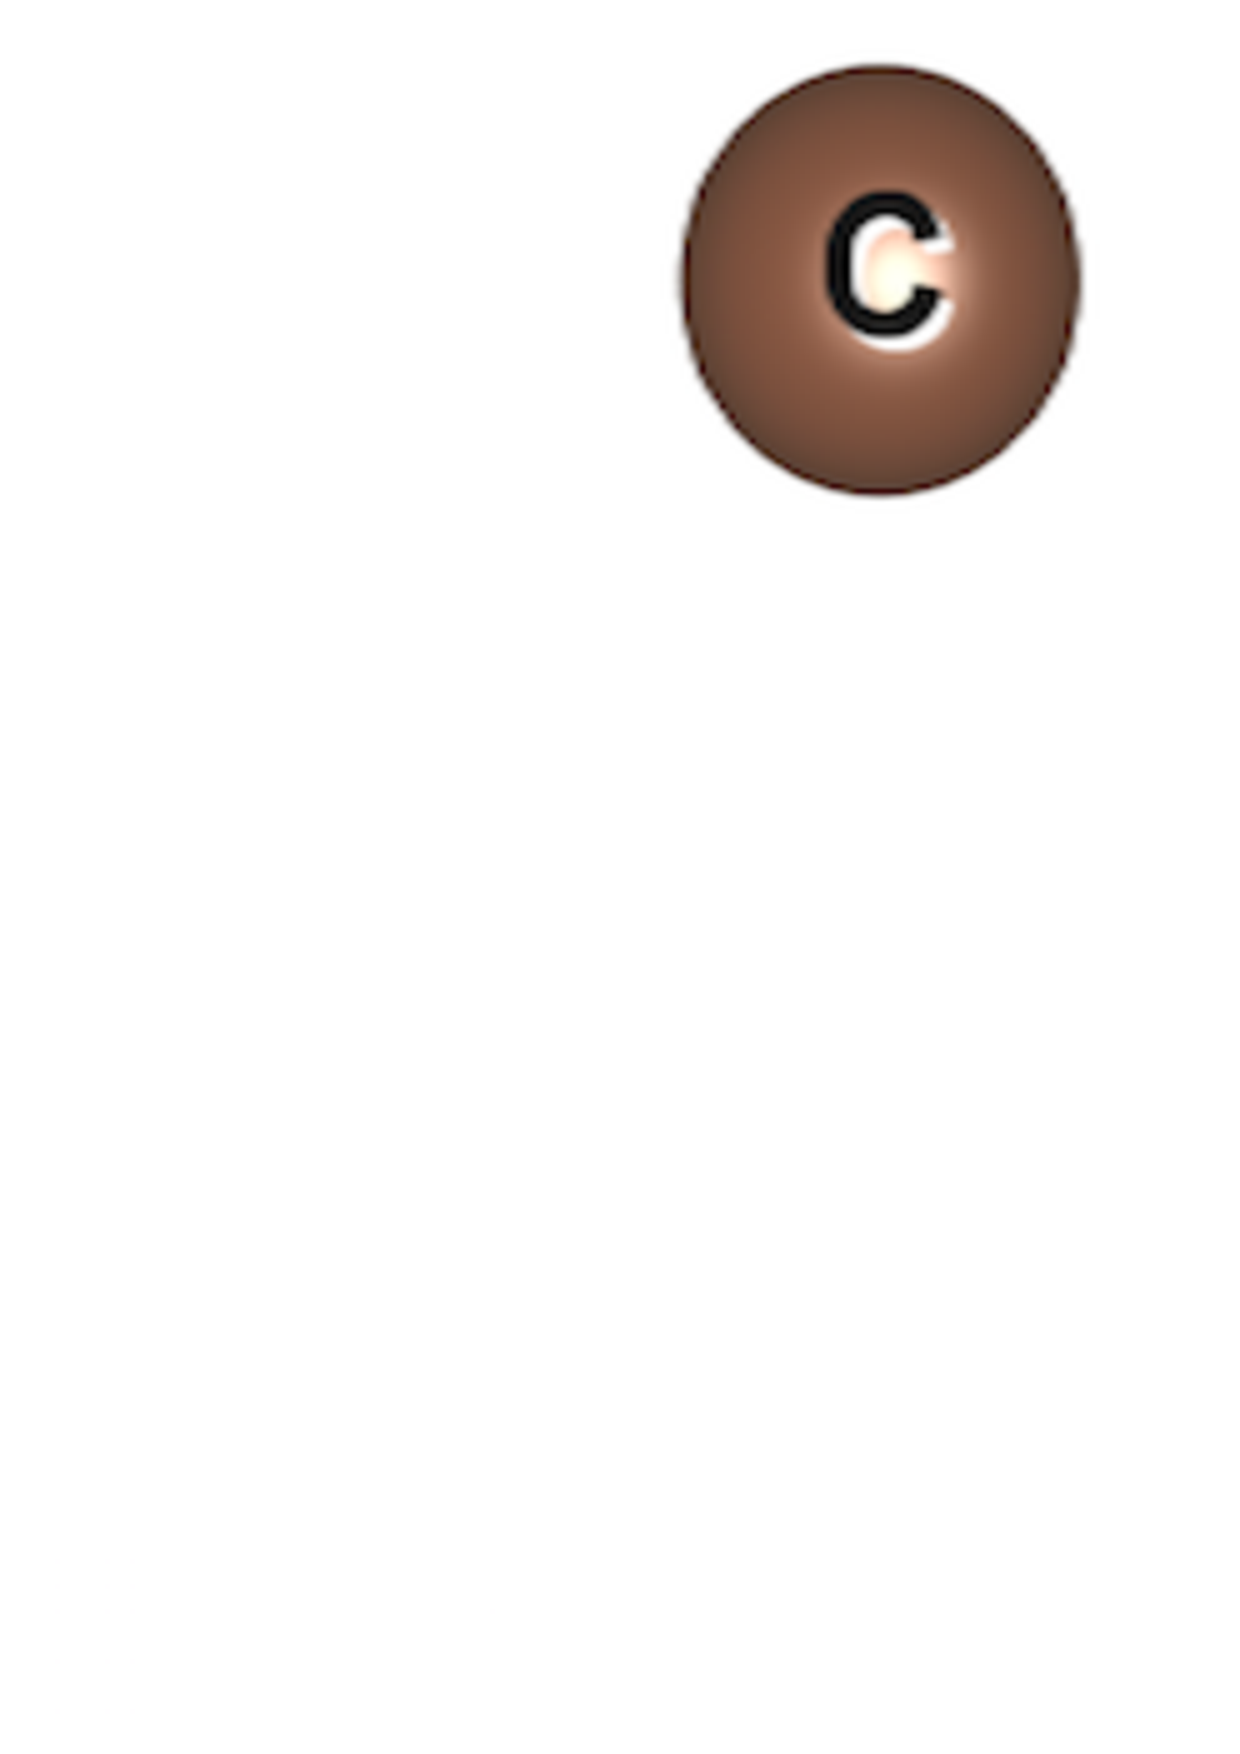
\includegraphics[clip, width=0.30\textwidth]{c_pi.png}}
    \subfigure[]{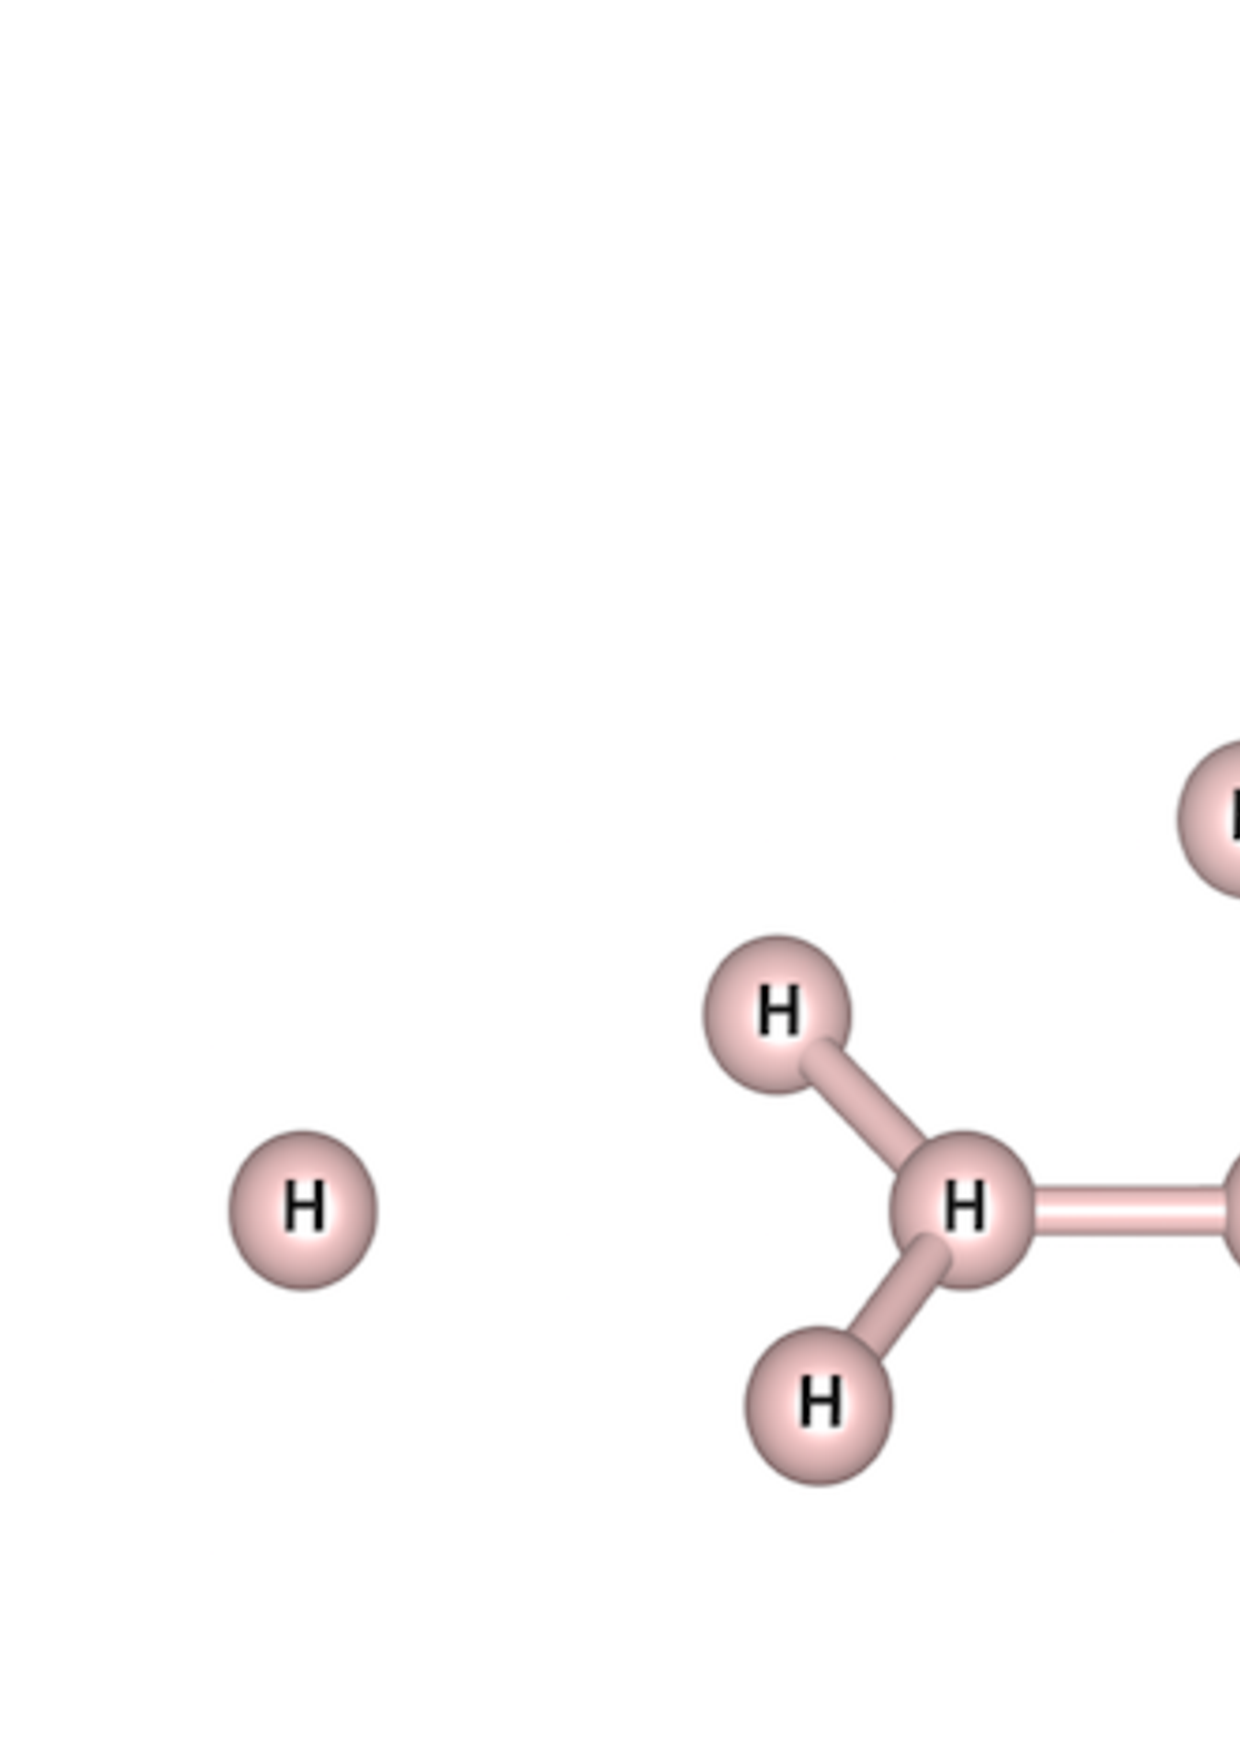
\includegraphics[clip, width=0.30\textwidth]{h_wan.png}}
       \caption{Wannier orbitals constructed from Kohn-Sham orbitals: (a) graphene $\pi$ orbitals; (b) hydrogen S orbital. }
\label{fig:wan}
\end{figure*}

We will use the non-eigenstate AIDMD method to obtain the value of $t$ and $U$. In this way, we do not need to solve the model Hamiltonian which is relatively difficult. We choose a set of Slater-Jastrow wave functions corresponding to the electron-hole excitations within the $\pi$ channel (or $s$ channel for hydrogen system). The energy expectation expressed in terms of the density matrices is, 
\begin{eqnarray}\label{eq:en}
E = C + t\sum_{\langle i, j\rangle, \sigma}( \rho_{ij}^\sigma + \rho_{ji}^\sigma) + U \sum_{i}M_{ii;ii}^{\uparrow,\downarrow}\,.
\end{eqnarray}

In order to understand the screening effect of $\sigma$ electrons, we also consider a $\pi$-only graphene, where we replace the $\sigma$ electrons with constant negative charge background. The lower energy states we choose for such systems are Slater-Jastrow wave functions constructed from occupied $\pi$ Kohn-Sham orbitals; whereas for the original graphene, the wave functions are Slater-Jastrow constructed from both occupied $\sigma$ bands and occupied $\pi$ bands. 

Table~\ref{tab:grpheffm} shows the final downfolding results of the three systems. The ab initio simulations are performed on a $3\times3$ cell. We have used using 25 low energy states for the downfolding. The error-bar is calculated using Jackniff method. 

\begin{table}[ht]
\label{tab:grpheffm}
\centering
\begin{tabular}{|c|c|c|c|}
\hline
parameters [eV] & graphene & $\pi$-only graphene &hydrogen \\
\hline
\hline
t & 3.61(1) & 2.99 & 3.73(1)\\
U & 7.16(3) & 14.8(2) & 9.47(5)\\
\hline
\end{tabular}
\caption{Downfolding parameters for graphene and hydrogen.}
\end{table} 
Fig.~\ref{fig:ne_aidmd_gh} shows fitted energies versus the \textit{ab initio} VMC energies. 

We find that the onsite Hubbard model describes graphene and hydrogen very well. The root mean square error of the predicted energies are relatively small (see Fig.~\ref{fig:ne_aidmd_gh}). The ratio of $U/t$ is small than the semi-metal-insulator transition critical value (3.8) in both graphene and hydrogen, which is consistent to the fact that both the two systems are semi-metals.  The $\pi$-only graphene however has larger $U/t$, and is in the insulating phase. This clearly shows the significance of $\sigma$ electrons in renormalizing the effective onsite interactions of $\pi$ orbitals. Without such screening effect, graphene will be an insulator. This is why many previous studies incorrectly predicted graphene to be an insulator in vacuum because they consider only $\pi$ electrons with bare Coulomb interaction \cite{DrutPRL2009, DrutPRB2009,  Smith2014}.

\begin{figure*}[htb]
\centering
\includegraphics[width=0.32\textwidth]{grp_all_tu.pdf}
\includegraphics[width=0.32\textwidth]{grp_pi_tu.pdf}
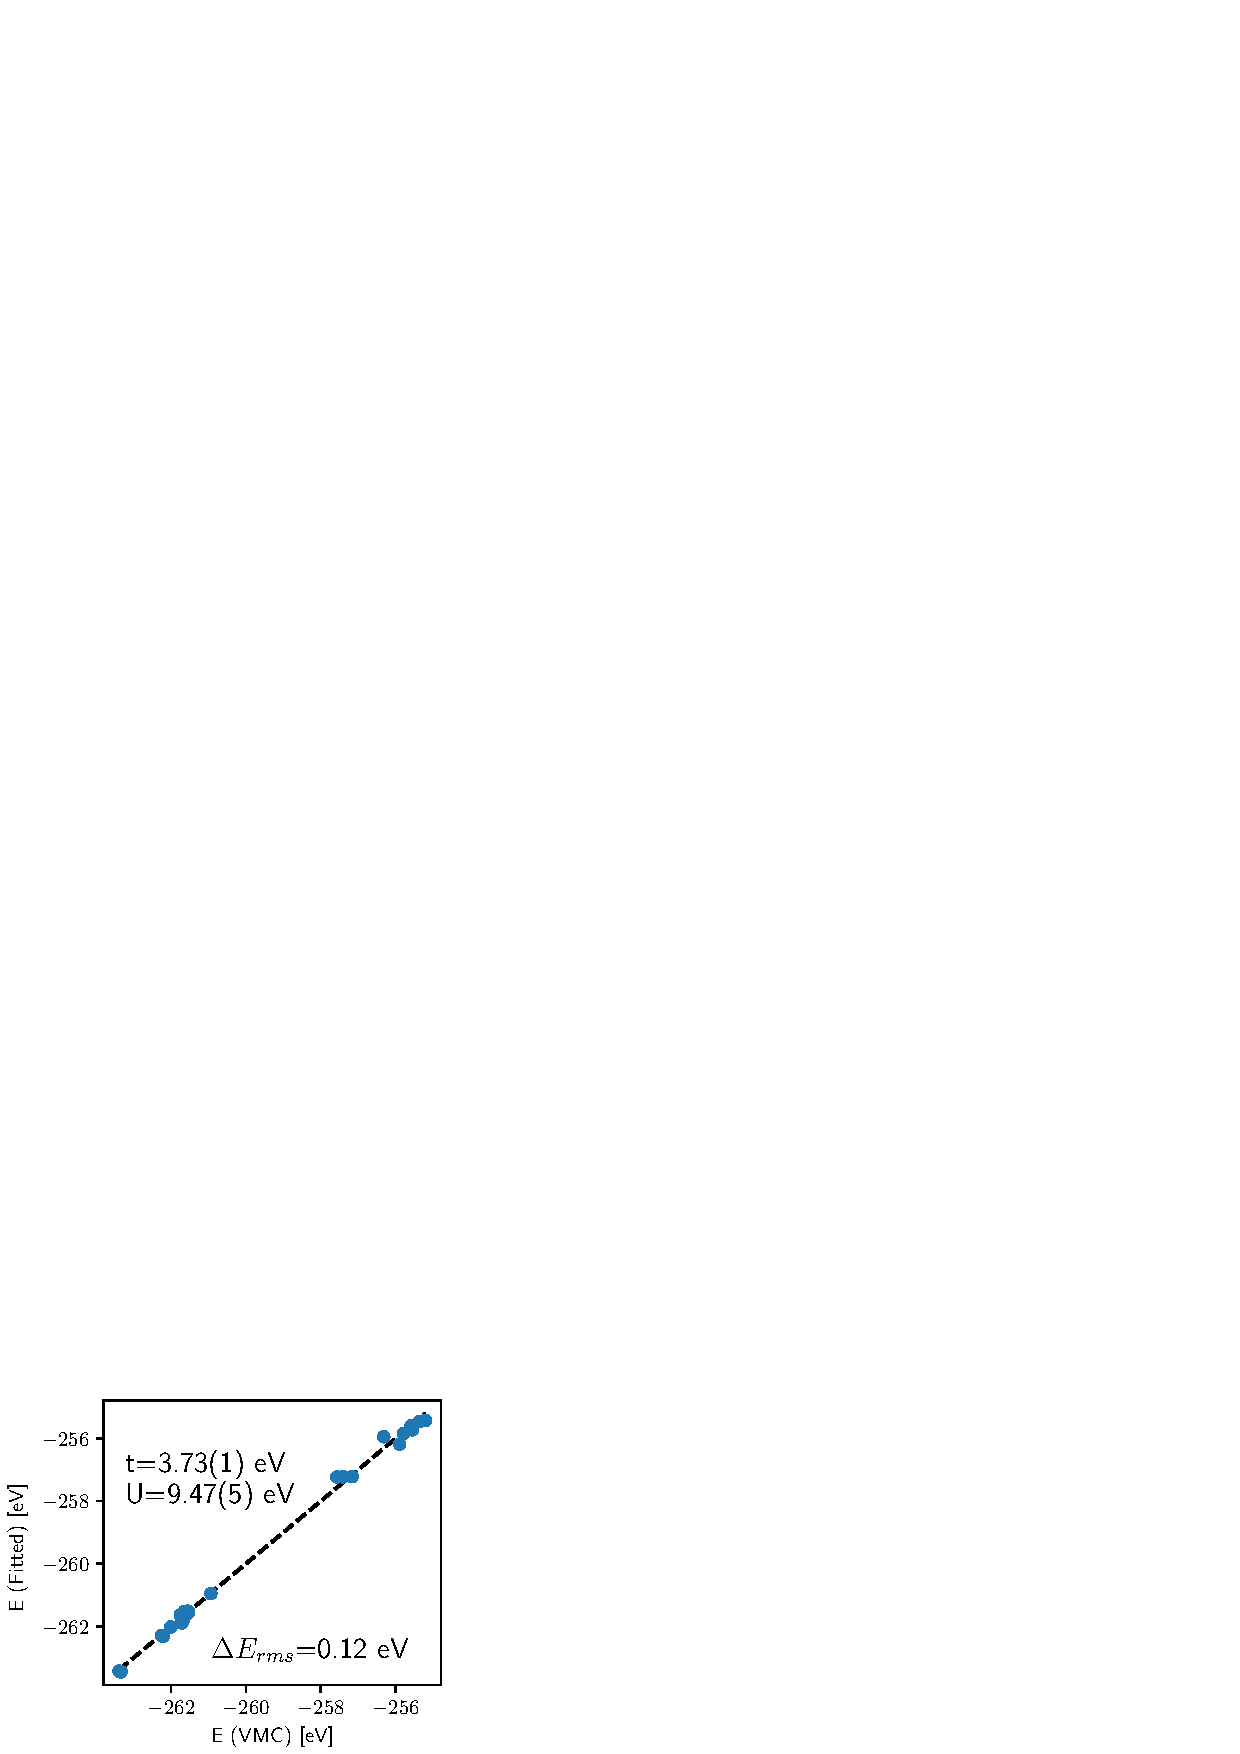
\includegraphics[width=0.32\textwidth]{h_tu.pdf}
\caption{Comparison of \textit{ab initio} (x-axis) and fitted energies (y-axis) of the 3$\times$3 periodic unit cell of graphene and hydrogen lattice: (a) graphene; (b) hydrogen lattice.}\label{fig:ne_aidmd_gh}
\end{figure*}

%\section{OTHER Realistic applications - silicon, carbon, transition metals, transition metal oxides}
%\HJC{LKW suggested silicon. This section is most uncertain. TM/ TMO stuff out}
\section{Prospects}
%\HJC{The need for including spin-orbit terms, need for QMC for this case}
\HJC{Other areas: Magnetism, can we access small energy scales? LKW suggests we can distinguish checkerboard vs Neel etc...}
\HJC{Applications to non QMC methods - coupled cluster, FCI, HCI}
\HJC{Strengths and limitations of effective Hamiltonian approach}

\bibliographystyle{unsrt}
\bibliography{refs}

\end{document}
